\labeledsection{Support Vector Machines}{sec:svm}
\titledbox{Remember}{
A line in 2D can be expressed as 
\[
ax + by + c = 0
\]
and the vector $\tuple{a,b}$ is the normal vector of that line (the one that is perpendicular (orthogonal) to the line (or any vector following the direction of the line))
}

\titledbox{Remember}{
Similarly, in 3D, a plane can be expressed as
\[
ax + by + cz + d = 0
\]
and the vector $\tuple{a,b,c}$ is the normal
}

In \linkterm{logistic regression}{logistic_regression_hypothesis}, we are trying to find the line that best separates two classes (assuming the data is \linkterm{linearly separable}{decision_boundary}),  we eventually find $w_1, w_2$ and find the line $w_1 x + w_2 y + b  = 0$ 

\commandnote{
The weight vector $\tuple{w_1, w_2}$ is orthogonal to that line 
}

\titledbox{Generalization}{
The equations used so far ($ax + by + c = 0$ for a line in 2D and $ax + by + cz + d = 0$ for a plane in 3D) work perfectly when the data has only 2 or 3 features. However, real-world datasets often have tens, hundreds, or thousands of features. 

To handle any number of dimensions cleanly without running out of alphabet letters for coordinates, vector dot products are used to represent the \linkterm{decision boundary}{decision_boundary} (the \linkterm{linear separator}{decision_boundary}).
}

\notationbox{
\begin{itemize}
    \item Instead of coordinate variables $(x, y, z, \dots)$, all features are packed into a single position vector: $\mathbf{x} = \tuple{x_1, x_2, \dots, x_d}^T$.
    \item Instead of individual coefficients $(a, b, c, \dots)$, all weights determining the tilt are packed into a single weight vector (the normal vector): $\mathbf{w} = \tuple{w_1, w_2, \dots, w_d}^T$.
    \item The standalone constant $b$ is retained as the scalar offset (bias) from the origin.
\end{itemize}
}

\anondefinition{
A \defemph{hyperplane} (the generalization of a line or a plane to $d$-dimensions) is formally defined as the set of all points $\mathbf{x}$ that satisfy the linear combination:
\[
\{ \mathbf{x} \mid (\mathbf{w} \cdot \mathbf{x}) + b = 0 \}
\]
where:
\begin{itemize}
    \item $\mathbf{w}$ is the weight vector, which stands completely \textbf{orthogonal} to the hyperplane, locking its orientation.
    \item $b$ is a scalar that determines the \textbf{offset} of the hyperplane from the origin.
\end{itemize}
}{hyperplane}

\problembox{
Which \linkterm{hyperplane}{hyperplane} (generalizes) well on unseen data ?
}
\begin{figure}[H]
    \centering
    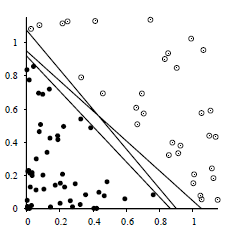
\includegraphics[width=0.2\linewidth]{images/which_line.png}
\end{figure}

\anondefinition{
Given a \linkterm{linearly separable}{decision_boundary} \linkterm{data set}{supervised_learning} $E$, the \defemph{maximum margin separator} is the \linkterm{linear separator}{decision_boundary} $s$ that maximizes the \defemph{margin} (the distance of the $E$ from $s$)
}{maximum_margin_separator}

\solutionbox{
The \linkterm{maximum margin separator}{maximum_margin_separator} generalizes best
}

\begin{figure}[H]
    \centering
    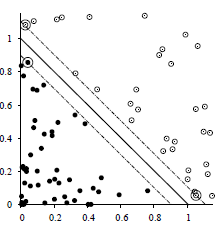
\includegraphics[width=0.2\linewidth]{images/maximum_margin_separator.png}
\end{figure}

\anondefinition{
\defemph{Support Vector Machines (SVMs)} are \linkterm{supervised learning}{supervised_learning} models for \linkterm{classification}{boolean_classification} and \linkterm{regression}{classifcation_regression}. \defemph{SVMs} construct a \linkterm{maximum margin separator}{maximum_margin_separator} by prioritizing critical \linkterm{examples}{supervised_learning} called \defemph{support vectors}
}{svm}

\begin{figure}[H]
    \centering
    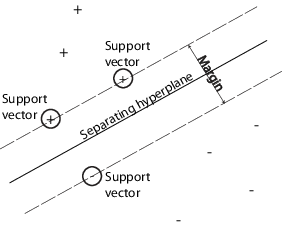
\includegraphics[width=0.2\linewidth]{images/support_vectors.png}
\end{figure}

\titledbox{Street Analogy}{
You can think of that as a street (with two gutters), where we want to maximize the distance between the gutters of the street
}

\notationbox{
We express classes as $\set{+1,-1}$ (positive and negative samples)
}

Once a hyperplane is fixed, it divides the entire feature space into two distinct regions. The weight vector $\mathbf{w}$ acts as a pointer, indicating which side is which.

\begin{itemize}
    \item \textbf{The Positive Half-Space:} Points falling on the side that $\mathbf{w}$ points toward will produce a positive result when plugged into the hyperplane equation.
    \item \textbf{The Negative Half-Space:} Points falling on the opposite side, away from the direction of $\mathbf{w}$, will produce a negative result.
\end{itemize}

\titledbox{Geometric Sign Rules}{
For any data point $\mathbf{x}$, its position relative to the hyperplane $\{\mathbf{x} \mid (\mathbf{w} \cdot \mathbf{x}) + b = 0\}$ determines the sign of the output:
\begin{align*}
(\mathbf{w} \cdot \mathbf{x}) + b > 0 & \quad \implies \quad \mathbf{x} \text{ lies on the \textbf{positive side} (in the direction of } \mathbf{w}\text{)} \\
(\mathbf{w} \cdot \mathbf{x}) + b < 0 & \quad \implies \quad \mathbf{x} \text{ lies on the \textbf{negative side} (opposite to } \mathbf{w}\text{)}
\end{align*}

We also need to allow $=$ to be on favor of the positive or negative class. Usually we say positive when $(\mathbf{w} \cdot \mathbf{x}) + b \geq 0$
}


\commandnote{
This behavior forms the basis of the SVM decision rule. By looking at the sign of $(\mathbf{w} \cdot \mathbf{x}) + b$, the model classifies the point as either $+1$ or $-1$.
}

\problembox{
We still do not know which $\mathbf{w}$ to use since we do not know the magnitude of that vector (we only know its orthogonal). And we do not know which offset $b$ to use.
}

\ideabox{
We need more constraints
}

\solutionbox{
We insist that positive samples need not just to be on the positive side of the \linkterm{decision boundary}{decision_boundary}, but they also need to be much further:
\[
\mathbf{w} \cdot \mathbf{x^{+}} + b \geq 1
\]

Similarly, for the negative samples:
\[
\mathbf{w} \cdot \mathbf{x^{-}} + b \leq -1
\]
}

\commandnote{
A positive sample $\mathbf{x_i^{+}}$ has $y_i = +1$ and a negative sample $\mathbf{x_i^{-}}$ has $y_i = -1$
}

\observationbox{
That means, we can combine these two constraints into a single elegant inequality by introducing the class label $y_i \in \{-1, +1\}$ for each sample $\mathbf{x}_i$:
\[
y_i (\mathbf{w} \cdot \mathbf{x}_i + b) \geq 1
\]
}

\Proof{
\begin{itemize}
    \item For positive samples, $y_i = +1$ and we trivially have $(\mathbf{w} \cdot \mathbf{x}_i + b) \geq 1$
    \item For negative samples, $y_i = -1$, we get $-(\mathbf{w} \cdot \mathbf{x}_i + b) \geq 1$
    \begin{itemize}
        \item We multiply or divide the whole inequality by $-1$, we get $(\mathbf{w} \cdot \mathbf{x}_i + b) \leq -1$
    \end{itemize}
\end{itemize}
}

\titledbox{New constraint}{
We can write the previous constraint compactly for all samples as:
\[
y_i (\mathbf{w} \cdot \mathbf{x}_i + b) - 1 \geq 0
\]
}

\commandnote{
We have imposed a strict separation zone where no data points are allowed to enter.
}

\questionbox{
Which samples satisfy this constraint with strict equality?
}

\answerbox{
The samples that lie \textbf{exactly on the boundaries} (the gutters of our street) will satisfy the constraint with strict equality ($= 0$). These critical points are the \linkterm{support vectors}{svm}:
\[
y_i (\mathbf{w} \cdot \mathbf{x}_i + b) - 1 = 0 \quad \implies \quad y_i (\mathbf{w} \cdot \mathbf{x}_i + b) = 1
\]
}

\titledbox{What do we have so far?}{
\begin{itemize}
    \item $\mathbf{w} \cdot \mathbf{x^{+}} + b > 1$ for safe positive samples
    \item $\mathbf{w} \cdot \mathbf{x^{-}} + b < -1$ for safe negative samples 
    \item $\mathbf{w} \cdot \mathbf{x_{sv}^{+}} + b = 1$ for positive support vectors (upper boundary)
    \item $\mathbf{w} \cdot \mathbf{x_{sv}^{-}} + b = -1$ for negative support vectors (lower boundary)
\end{itemize}
}

\begin{figure}[H]
    \centering
    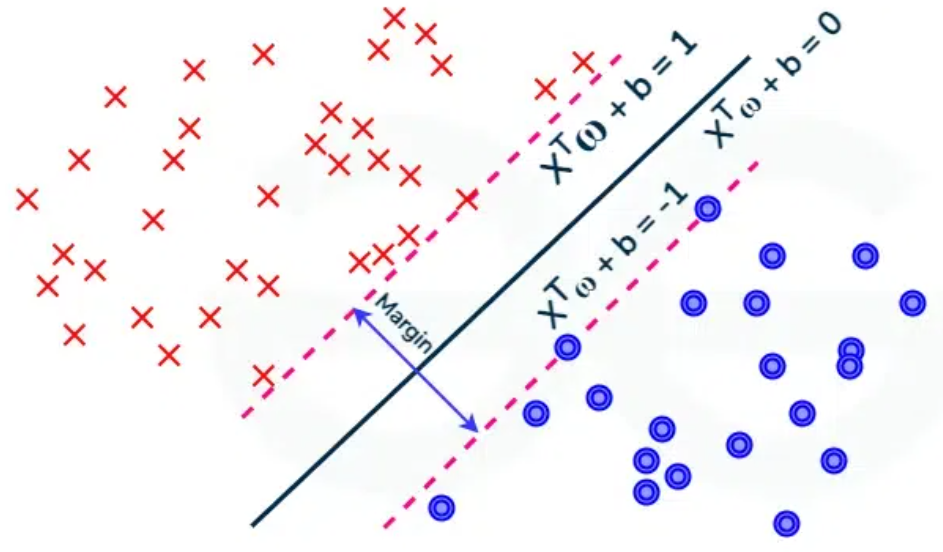
\includegraphics[width=0.3\linewidth]{images/constraints_svm.png}
\end{figure}

We expressed the first two as one constraint, and the second two as one constraint:
For all \linkterm{examples}{supervised_learning}, we have:
\begin{tcolorbox}[ams equation,colback=yellow!10!white,colframe=red!50!black]
y_i (\mathbf{w} \cdot \mathbf{x}_i + b) - 1 \geq 0 \label{eq:allsamplesconst}
\end{tcolorbox}

For the \linkterm{support vectors}{svm} (special examples), we have:
\begin{tcolorbox}[ams equation,colback=yellow!10!white,colframe=red!50!black]
y_i (\mathbf{w} \cdot \mathbf{x}_i + b) - 1 = 0 \label{eq:gutterconst}
\end{tcolorbox}

\titledbox{Remember}{
We are trying to find the line that separates the positives from negatives as wide as possible
}

\questionbox{
How to calculate the width of the street ?
}

\newpage
Imagine the following situation. We have a vector representing a negative example $\tuple{2,4}$ exactly on the lower boundary (a negative support vector) and we have a positive support vector too $\tuple{5,6}$. 

\begin{figure}[H]
    \centering
    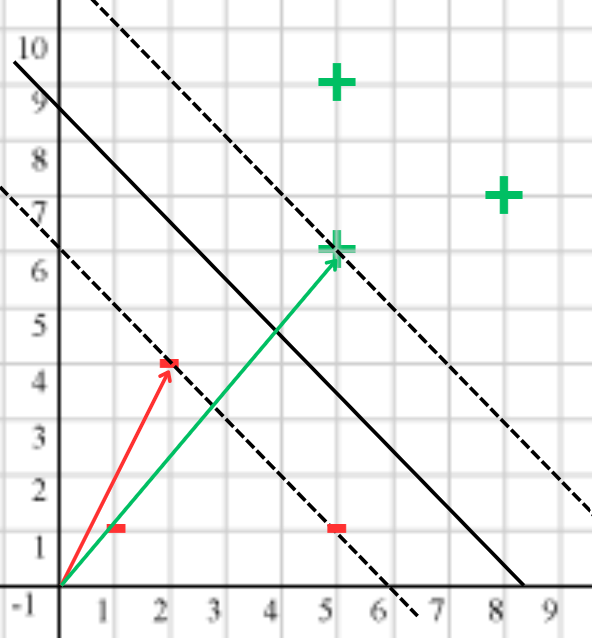
\includegraphics[width=0.3\linewidth]{images/svm1.png}
\end{figure}

If we subtract the negative form the positive, we get:
\[
\mathbf{x}_{+} - \mathbf{x}_{-} = \tuple{3,2}
\]

\begin{figure}[H]
    \centering
    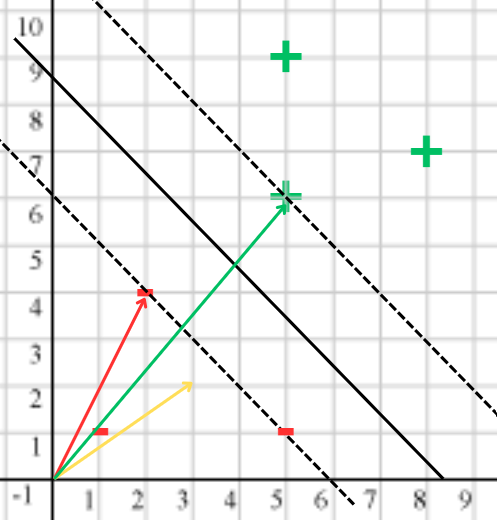
\includegraphics[width=0.3\linewidth]{images/svm2.png}
\end{figure}

If we take that and place it between the tips of the two support vectors, we have:

\begin{figure}[H]
    \centering
    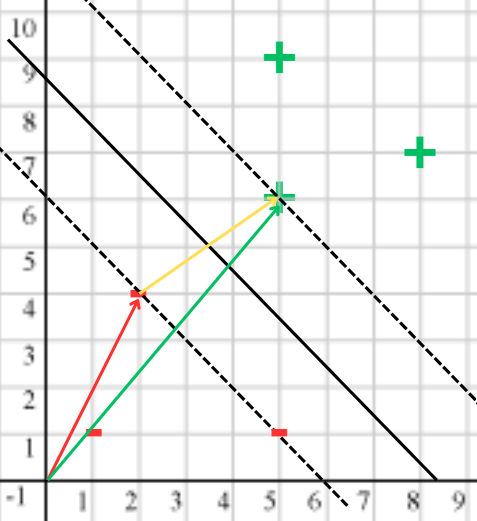
\includegraphics[width=0.3\linewidth]{images/svm3.png}
\end{figure}

If we have a unit vector that is normal to our line (or the gutters):
\begin{figure}[H]
    \centering
    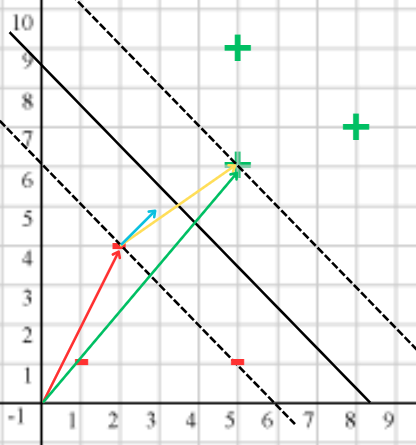
\includegraphics[width=0.3\linewidth]{images/svm4.png}
\end{figure}

then we can dot product the unit normal (blue) with the difference vector (yellow), and we get a vector that its magnitude is exactly the total width that we want to maximize!
\begin{figure}[H]
    \centering
    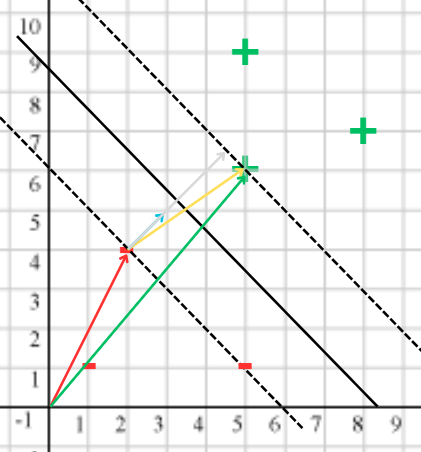
\includegraphics[width=0.3\linewidth]{images/svm5.png}
\end{figure}

\observationbox{
The weight vector $\mathbf{w}$ is a normal vector!
}

\ideabox{
Make $\mathbf{w}$ a unit vector.
}

\commandnote{
We can make any vector $\mathbf{x}$ a unit vector by dividing it by its magnitude:
\[
\frac{\mathbf{x}}{\norm{\mathbf{x}}}
\]
}

\redbox{
The width of our (street) is:
\[
(\mathbf{x}_{+} - \mathbf{x}_{-}) \cdot \frac{\mathbf{w}}{\norm{\mathbf{w}}}
\]
}

\observationbox{
\begin{itemize}
    \item From \Eqref{eq:gutterconst}, we know that $\mathbf{x}_{+} \cdot \mathbf{w} = 1-b$
    \item We also know that $-\mathbf{x}_{-} \cdot \mathbf{w} = 1 + b$
\end{itemize}
}

Therefore, we can write our width as:
\begin{align*}
\text{Width} &= (\mathbf{x}_{+} - \mathbf{x}_{-}) \cdot \frac{\mathbf{w}}{\norm{\mathbf{w}}} \\ 
 &= (\mathbf{x}_{+} \cdot \mathbf{w} - \mathbf{x}_{-} \cdot \mathbf{w}) \cdot \frac{1}{\norm{\mathbf{w}}} \\ 
 &= (1-b + 1 + b) \cdot \frac{1}{\norm{\mathbf{w}}} \\ 
 &= 2 \cdot \frac{1}{\norm{\mathbf{w}}} \\ 
\text{Width} &= \frac{2}{\norm{\mathbf{w}}} 
\end{align*}

\titledbox{Mathematical Convenience}{
We want to maximize $\frac{2}{\norm{\mathbf{w}}}$, which also mean we can maximize $\frac{1}{\norm{\mathbf{w}}}$, which we can do by \textbf{minimizing} $\norm{\mathbf{w}}$.

For convenience, the goal becomes to \textbf{minimize} $\frac{1}{2}\norm{\mathbf{w}}^2$
}

\titledbox{Constrained Optimization Problem}{
We are left with the following constrained optimization problem:
\[
\argmin{\mathbf{w}, b} \frac{1}{2}\norm{\mathbf{w}}^2
\]
subject to \Eqref{eq:allsamplesconst} for all $i = 1, \dots, N$.
}

\problembox{
We cannot solve this optimization problem using standard calculus (like setting the derivative to zero) because of the inequality constraints. The optimal unconstrained solution for $\frac{1}{2}\norm{\mathbf{w}}^2$ is simply $\mathbf{w} = \mathbf{0}$, which completely fails to separate our data.
}

\ideabox{
We need a mathematical framework that allows us to optimize our objective function while strictly enforcing that every single data point stays on or outside the gutter boundaries.
}

\anondefinition{
The method of \defemph{Lagrange Multipliers} is a strategy used in calculus to find the local maxima and minima of a function subject to constraints. It works by combining the original objective function and the constraints into a single equation called the \defemph{Lagrangian}.
}{lagrange_multipliers}

\commandnote{
For every constraint in our dataset, we introduce a new variable called a Lagrange multiplier, denoted as $\alpha_i \geq 0$. 
\begin{itemize}
    \item If a sample is safely past the gutter, its constraint is satisfied easily, and its multiplier $\alpha_i$ will be $0$.
    \item If a sample is a critical \linkterm{support vector}{svm} sitting exactly on the gutter, its multiplier $\alpha_i$ will be greater than $0$.
\end{itemize}
}

\titledbox{The Primal Lagrangian Function}{
By introducing a multiplier $\alpha_i$ for each of our $N$ constraints from \Eqref{eq:allsamplesconst}, we construct the Primal Lagrangian function $L_p$:
\[
L_p(\mathbf{w}, b, \boldsymbol{\alpha}) = \frac{1}{2}\norm{\mathbf{w}}^2 - \sum_{i=1}^{N} \alpha_i \left[ y_i (\mathbf{w} \cdot \mathbf{x}_i + b) - 1 \right]
\]
Our goal is to find the saddle point: minimizing this function with respect to $\mathbf{w}$ and $b$, while maximizing it with respect to $\boldsymbol{\alpha}$.
}

\anondefinition{
A \defemph{saddle point} is a point on a function's surface where the slopes (derivatives) in all orthogonal directions are zero, but which is a local minimum along one cross-section and a local maximum along another.
}{saddle_point}

\begin{figure}[H]
    \centering
    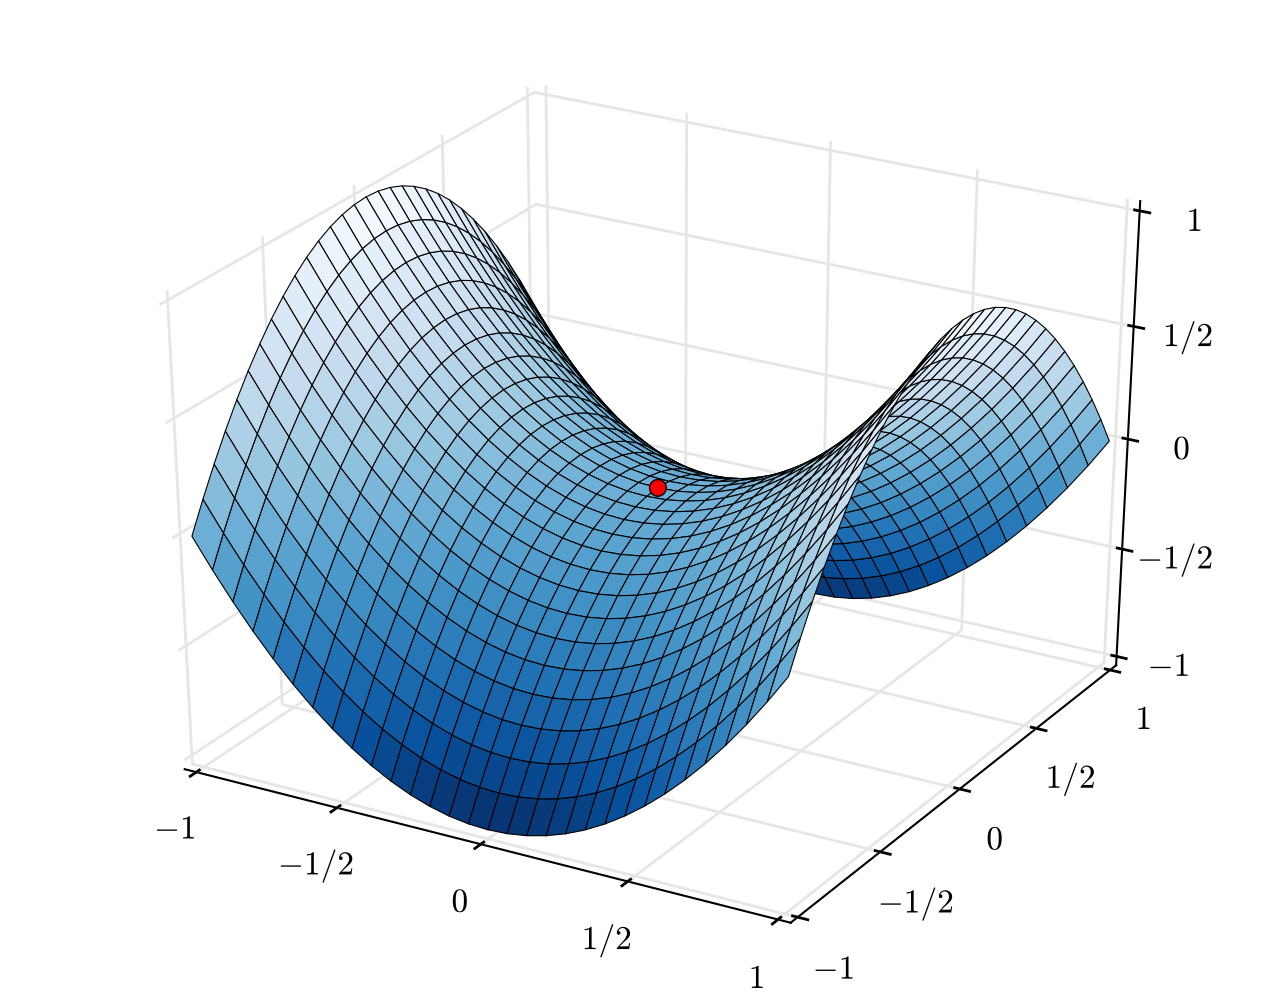
\includegraphics[width=0.3\linewidth]{images/Saddle_point.png}
\end{figure}


\observationbox{
In our Primal Lagrangian $L_p(\mathbf{w}, b, \boldsymbol{\alpha})$:
\begin{itemize}
    \item We want to \textbf{minimize} with respect to the model parameters $\mathbf{w}$ and $b$ to find the cleanest separating line.
    \item We want to \textbf{maximize} with respect to the Lagrange multipliers $\boldsymbol{\alpha}$ to strictly penalize any constraint violations.
\end{itemize}
At the optimal solution, we land exactly at this balanced saddle point.
}

\questionbox{
How do we find this saddle point mathematically?
}

\answerbox{
Since the Lagrangian is convex with respect to $\mathbf{w}$ and $b$, we can find the minimum by taking the partial derivatives with respect to $\mathbf{w}$ and $b$, setting them to zero:
\[
\frac{\partial L_p}{\partial \mathbf{w}} = 0 \quad \text{and} \quad \frac{\partial L_p}{\partial b} = 0
\]
}

\questionbox{
Why are we allowed to just take the partial derivatives and set them to zero?
}

\answerbox{
We can do this because the Primal Lagrangian $L_p(\mathbf{w}, b, \boldsymbol{\alpha})$ is \textbf{strictly convex} with respect to $\mathbf{w}$ and \textbf{linear} (convex) with respect to $b$. This guarantees that any local minimum we find is the unique global minimum.
}

To see why, we break the Lagrangian into its two distinct algebraic components:
\[
L_p(\mathbf{w}, b, \boldsymbol{\alpha}) = \underbrace{\frac{1}{2}\norm{\mathbf{w}}^2}_{\text{Part 1: Objective}} - \underbrace{\sum_{i=1}^{N} \alpha_i \left[ y_i (\mathbf{w} \cdot \mathbf{x}_i + b) - 1 \right]}_{\text{Part 2: Constraints}}
\]

\titledbox{Component Breakdown}{
\begin{enumerate}
    \item \textbf{Part 1 (The Objective Function):} The term $\frac{1}{2}\norm{\mathbf{w}}^2 = \frac{1}{2}(w_1^2 + w_2^2 + \dots + w_d^2)$ is a squared Euclidean norm. Geometrically, this shapes a perfect multi-dimensional bowl (\textit{paraboloid}), which is strictly convex.
    \item \textbf{Part 2 (The Constraints):} The optimization variables $\mathbf{w}$ and $b$ only appear as first-power terms ($\mathbf{w}^1$ and $b^1$) with no cross-multiplications. This forms a \textbf{linear function} (a perfectly flat sheet), which possesses zero curvature and is inherently convex.
\end{enumerate}
}

\begin{figure}[H]
    \centering
    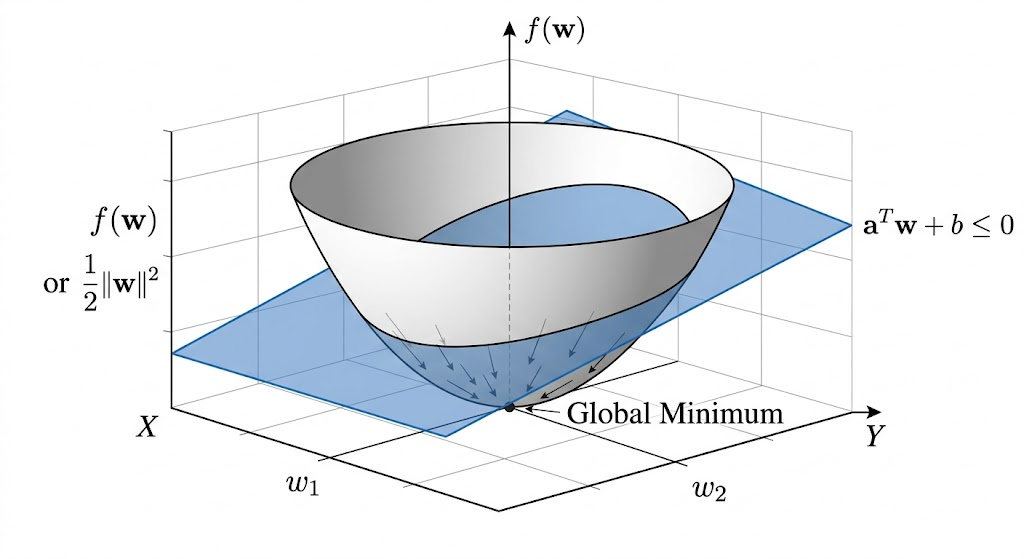
\includegraphics[width=0.4\linewidth]{images/convex_bowl.png}
    \caption{Adding a flat linear sheet to a strictly convex bowl preserves the bowl shape, keeping the entire surface convex.}
\end{figure}

\observationbox{
Since the sum of two convex functions is always convex, the entire surface forms a predictable bowl along the $\mathbf{w}$ and $b$ axes. This structural guarantee is what justifies setting the partial derivatives to zero:
\[
\nabla_{\mathbf{w}} L_p = \mathbf{0} \quad \text{and} \quad \frac{\partial L_p}{\partial b} = 0
\]
\label{obs:convexity_justification}
}

To find the optimal weight vector $\mathbf{w}$ at our saddle point, we take the partial derivative of the Primal Lagrangian $L_p$ with respect to $\mathbf{w}$ and set it to zero. 

Let's first expand $L_p$ to isolate the terms containing $\mathbf{w}$:
\[
L_p(\mathbf{w}, b, \boldsymbol{\alpha}) = \frac{1}{2}\norm{\mathbf{w}}^2 - \sum_{i=1}^{N} \alpha_i y_i (\mathbf{w} \cdot \mathbf{x}_i) - \sum_{i=1}^{N} \alpha_i y_i b + \sum_{i=1}^{N} \alpha_i
\]

\questionbox{
How do we compute the gradient component by component?
}

\answerbox{
We differentiate the two relevant terms independently using matrix/vector calculus identities:
\begin{enumerate}
    \item \textbf{The Objective Term:} Since $\norm{\mathbf{w}}^2 = \mathbf{w} \cdot \mathbf{w}$, its gradient with respect to $\mathbf{w}$ is:
    \[
    \frac{\partial}{\partial \mathbf{w}} \left( \frac{1}{2}\norm{\mathbf{w}}^2 \right) = \mathbf{w}
    \]
    \item \textbf{The Constraint Term:} Since the dot product is linear ($\frac{\partial}{\partial \mathbf{w}}(\mathbf{w} \cdot \mathbf{x}_i) = \mathbf{x}_i$), the summation terms differentiate to:
    \[
    \frac{\partial}{\partial \mathbf{w}} \left( \sum_{i=1}^{N} \alpha_i y_i (\mathbf{w} \cdot \mathbf{x}_i) \right) = \sum_{i=1}^{N} \alpha_i y_i \mathbf{x}_i
    \]
\end{enumerate}
}

Combining these results, we get the complete gradient expression:
\begin{align*}
\frac{\partial L_p}{\partial \mathbf{w}} &= \mathbf{w} - \sum_{i=1}^{N} \alpha_i y_i \mathbf{x}_i = \mathbf{0}
\end{align*}

\redbox{
By solving for $\mathbf{w}$, we discover that the optimal weight vector is a linear combination of our training samples:
\[
\mathbf{w} = \sum_{i=1}^{N} \alpha_i y_i \mathbf{x}_i
\]
}

\observationbox{
This is a beautiful conceptual milestone! It proves that the normal vector $\mathbf{w}$ defining the optimal hyperplane is completely constructed from the data points themselves. Furthermore, because non-support vectors have $\alpha_i = 0$, $\mathbf{w}$ is entirely determined \textit{only} by the support vectors.
}

Next, we look at how the Primal Lagrangian changes with respect to our scalar offset, the bias $b$. We take the partial derivative of $L_p$ with respect to $b$ and set it to zero.

Let's revisit the expanded Lagrangian to see exactly where $b$ appears:
\[
L_p(\mathbf{w}, b, \boldsymbol{\alpha}) = \frac{1}{2}\norm{\mathbf{w}}^2 - \sum_{i=1}^{N} \alpha_i y_i (\mathbf{w} \cdot \mathbf{x}_i) - \sum_{i=1}^{N} \alpha_i y_i b + \sum_{i=1}^{N} \alpha_i
\]

\questionbox{
How does the summation collapse during differentiation?
}

\answerbox{
Since $b$ appears strictly as a first-power scalar linear term, any term lacking $b$ disappears. Moving the derivative inside the summation yields:
\[
\frac{\partial L_p}{\partial b} = -\sum_{i=1}^{N} \alpha_i y_i \frac{\partial}{\partial b}(b) = -\sum_{i=1}^{N} \alpha_i y_i 
\]
}

Setting this result to zero gives us our complete derivative expression:
\begin{align*}
\frac{\partial L_p}{\partial b} &= -\sum_{i=1}^{N} \alpha_i y_i = 0
\end{align*}

\redbox{
By multiplying by $-1$, we uncover an incredibly strict constraint on our Lagrange multipliers:
\begin{equation}
    \sum_{i=1}^{N} \alpha_i y_i = 0 \label{eq:optimal_b_condition}
\end{equation}
}

\observationbox{
This constraint tells us that the weighted sum of our labels multiplied by their Lagrange multipliers must perfectly balance out to zero. It acts as an equilibrium condition for the optimization problem. When we transition to the Dual Lagrangian, this relation will allow us to completely eliminate the parameter $b$ from the objective function!
}

Now that we have expressions for our optimal parameters, we begin the transition to the Dual Lagrangian by substituting $\mathbf{w} = \sum_{i=1}^{N} \alpha_i y_i \mathbf{x}_i$ back into the Primal Lagrangian function $L_p$.

Let's carefully observe the substitution for the first two terms of $L_p$:

\titledbox{Step-by-Step Substitution}{
\begin{enumerate}
    \item \textbf{The Squared Norm Term:} Writing $\norm{\mathbf{w}}^2$ as a dot product requires utilizing two independent indices ($i$ and $j$) to track the cross-multiplications:
    \[
    \frac{1}{2}\norm{\mathbf{w}}^2 = \frac{1}{2} \left( \sum_{i=1}^{N} \alpha_i y_i \mathbf{x}_i \right) \cdot \left( \sum_{j=1}^{N} \alpha_j y_j \mathbf{x}_j \right) = \frac{1}{2} \sum_{i=1}^{N} \sum_{j=1}^{N} \alpha_i \alpha_j y_i y_j (\mathbf{x}_i \cdot \mathbf{x}_j)
    \]
    \item \textbf{The Interaction Term:} Substituting $\mathbf{w}$ into the constraint summation yields an identical double summation structure:
    \[
    \sum_{i=1}^{N} \alpha_i y_i (\mathbf{w} \cdot \mathbf{x}_i) = \sum_{i=1}^{N} \alpha_i y_i \left( \sum_{j=1}^{N} \alpha_j y_j \mathbf{x}_j \cdot \mathbf{x}_i \right) = \sum_{i=1}^{N} \sum_{j=1}^{N} \alpha_i \alpha_j y_i y_j (\mathbf{x}_i \cdot \mathbf{x}_j)
    \]
\end{enumerate}
}

\questionbox{
How do these two expanded double sums combine?
}

\answerbox{
Since the second double sum is exactly identical to the first, subtracting them simplifies beautifully like a simple fraction ($\frac{1}{2}A - 1A = -\frac{1}{2}A$):
\[
\frac{1}{2}\norm{\mathbf{w}}^2 - \sum_{i=1}^{N} \alpha_i y_i (\mathbf{w} \cdot \mathbf{x}_i) = -\frac{1}{2} \sum_{i=1}^{N} \sum_{j=1}^{N} \alpha_i \alpha_j y_i y_j (\mathbf{x}_i \cdot \mathbf{x}_j)
\]
}

Our updated Lagrangian function now reads:
\[
L_p(b, \boldsymbol{\alpha}) = -\frac{1}{2} \sum_{i=1}^{N} \sum_{j=1}^{N} \alpha_i \alpha_j y_i y_j (\mathbf{x}_i \cdot \mathbf{x}_j) - b\sum_{i=1}^{N} \alpha_i y_i + \sum_{i=1}^{N} \alpha_i
\]


The final step in our transition is to apply the equilibrium condition derived from the bias parameter. 

Recall our current state of the Lagrangian:
\[
L_p(b, \boldsymbol{\alpha}) = -\frac{1}{2} \sum_{i=1}^{N} \sum_{j=1}^{N} \alpha_i \alpha_j y_i y_j (\mathbf{x}_i \cdot \mathbf{x}_j) - b\sum_{i=1}^{N} \alpha_i y_i + \sum_{i=1}^{N} \alpha_i
\]

\questionbox{
What happens to the parameter $b$?
}

\answerbox{
From \Eqref{eq:optimal_b_condition}, we established that $\sum_{i=1}^{N} \alpha_i y_i = 0$. Substituting this identity directly into the equation forces the dependency on $b$ to vanish entirely:
\[
-b \cdot \left( \sum_{i=1}^{N} \alpha_i y_i \right) = -b \cdot (0) = 0
\]
}

\titledbox{The Dual Optimization Problem}{
By removing $b$, we arrive at the \textbf{Dual Lagrangian Function} $L_d(\boldsymbol{\alpha})$, which we rearrange to list the positive linear term first:
\[
L_d(\boldsymbol{\alpha}) = \sum_{i=1}^{N} \alpha_i - \frac{1}{2} \sum_{i=1}^{N} \sum_{j=1}^{N} \alpha_i \alpha_j y_i y_j (\mathbf{x}_i \cdot \mathbf{x}_j)
\]
We can now state the complete Dual Optimization problem:
\[
\argmax{\boldsymbol{\alpha}} \left( \sum_{i=1}^{N} \alpha_i - \frac{1}{2} \sum_{i=1}^{N} \sum_{j=1}^{N} \alpha_i \alpha_j y_i y_j (\mathbf{x}_i \cdot \mathbf{x}_j) \right)
\]
\[
\text{subject to } \alpha_i \geq 0 \quad \text{for all } i, \quad \text{and} \quad \sum_{i=1}^{N} \alpha_i y_i = 0
\]
}

\observationbox{
Look at how elegant this formulation is! The optimization problem no longer cares about the dimensionality of our feature vectors $\mathbf{x}_i$. The data only enters the calculation via the \textbf{dot product} $\mathbf{x}_i \cdot \mathbf{x}_j$, which computes the similarity between every pair of samples. This structural property is what completely unlocks the potential of non-linear kernels.
}

Remember our decision rule, we say that an unknown sample $\mathbf{u}$ is positive if:
\[
(\mathbf{w} \cdot \mathbf{u}) + b \geq 0
\]
And we figured out that
\[
\mathbf{w} = \sum_{i=1}^{N} \alpha_i y_i \mathbf{x}_i
\]

So the decision rule becomes:
\[
(\sum_{i=1}^{N} \alpha_i y_i \mathbf{x}_i \cdot \mathbf{u}) + b \geq 0
\]

\commandnote{
The decision rule also depends only on the dot product of our sample vectors with the unknown sample $\mathbf{u}$
}

\problembox{
What if the \linkterm{data set}{supervised_learning} is not \linkterm{linearly separable}{decision_boundary} ?
}


When a dataset is completely twisted, clustered, or non-linear, no flat hyperplane in our current space can separate it. To solve this, we can shift our perspective entirely: we map our low-dimensional data into a much higher-dimensional space where the data naturally untangles and becomes linearly separable. 

Once we find the separating hyperplane in that high-dimensional space, projecting the boundary back down to our original space yields a highly flexible, non-linear decision boundary.

\begin{figure}[H]
    \centering
    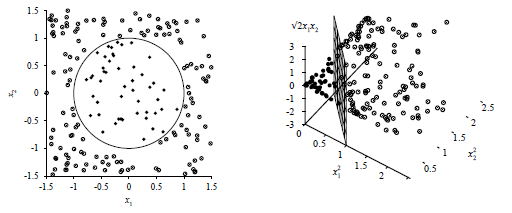
\includegraphics[width=0.45\linewidth]{images/kernel_mapping.png}
\end{figure}


\anondefinition{
A \defemph{Feature Map} is a function $\Phi: \mathbb{R}^d \to \mathbb{R}^D$ (where $D \gg d$) that takes a vector from the original input space and projects it into a higher-dimensional feature space.
}{feature_map}

If we apply this feature map to our entire derivation, every single occurrence of an input vector $\mathbf{x}$ is replaced by its higher-dimensional counterpart $\Phi(\mathbf{x})$. 

Our Dual Optimization objective becomes:
\[
\argmax{\boldsymbol{\alpha}} \left( \sum_{i=1}^{N} \alpha_i - \frac{1}{2} \sum_{i=1}^{N} \sum_{j=1}^{N} \alpha_i \alpha_j y_i y_j \mathbf{\Phi}(\mathbf{x}_i) \cdot \mathbf{\Phi}(\mathbf{x}_j) \right)
\]

And our corresponding decision rule updates to:
\[
\sum_{i=1}^{N} \alpha_i y_i \mathbf{\Phi}(\mathbf{x}_i) \cdot \mathbf{\Phi}(\mathbf{u}) + b \geq 0
\]

\problembox{
Computing $\Phi(\mathbf{x})$ explicitly is incredibly expensive. If we map our data into an infinite-dimensional space, the vector $\Phi(\mathbf{x})$ has infinite coordinates, making it mathematically impossible to compute or store in memory!
}

\ideabox{
Look closely at the updated equations. We never actually need to know the isolated coordinates of the high-dimensional vector $\Phi(\mathbf{x})$. The data \textbf{only} interacts through the dot product $\Phi(\mathbf{x}_i) \cdot \Phi(\mathbf{x}_j)$, which outputs a simple, scalar similarity score!
}

What if we could compute that final scalar similarity score directly using an easy function in our original low-dimensional space, without ever calculating the massive vector $\Phi(\mathbf{x})$? This is the core realization behind the Kernel Trick.

\anondefinition{
The \defemph{Kernel Trick} is an optimization shortcut where a function $K(\mathbf{x}_i, \mathbf{x}_j)$ computes the inner product of vectors in a higher-dimensional feature space directly in the input space, bypassing the explicit computation of the high-dimensional coordinates:
\[
K(\mathbf{x}_i, \mathbf{x}_j) = \mathbf{\Phi}(\mathbf{x}_i) \cdot \mathbf{\Phi}(\mathbf{x}_j)
\]
}{kernel_trick}

By using a predefined kernel function $K$, our training objective and decision rule simplify perfectly:
\[
\text{Objective: } \argmax{\boldsymbol{\alpha}} \left( \sum_{i=1}^{N} \alpha_i - \frac{1}{2} \sum_{i=1}^{N} \sum_{j=1}^{N} \alpha_i \alpha_j y_i y_j K(\mathbf{x}_i, \mathbf{x}_j) \right)
\]
\[
\text{Decision Rule: } \sum_{i=1}^{N} \alpha_i y_i K(\mathbf{x}_i, \mathbf{u}) + b \geq 0
\]


\commandnote{
We do not need to invent a mapping function $\Phi(\mathbf{x})$ from scratch. Instead, we can choose from a set of mathematically validated kernel functions that implicitly define different high-dimensional geometries.
}

\textbf{1. The Polynomial Kernel}

The Polynomial kernel explicitly represents similarities up to a specific degree of feature interactions (like cross-terms $x_1x_2$).

\begin{tcolorbox}[colback=blue!5!white,colframe=blue!75!black,title=Polynomial Kernel Formula]
\[
K(\mathbf{x}, \mathbf{z}) = (\mathbf{x} \cdot \mathbf{z} + c)^d
\]
Where $d$ is the polynomial degree and $c \geq 0$ is a tuning constant trading off the influence of higher-order versus lower-order terms.
\end{tcolorbox}

\textbf{How it works:} If $d=2$ and $c=0$ in a 2D space, computing $K(\mathbf{x}, \mathbf{z}) = (\mathbf{x} \cdot \mathbf{z})^2$ is equivalent to mapping the data into a 3D space using $\Phi(\mathbf{x}) = \langle w_1^2, \sqrt{2}w_1w_2, w_2^2 \rangle$. It allows the boundary to form perfect parabolas, ellipses, or hyperbolas in the original space.

\textbf{2. The Radial Basis Function (RBF) / Gaussian Kernel}

The RBF kernel is the most popular kernel in machine learning. It acts as a local similarity metric.

\begin{tcolorbox}[colback=blue!5!white,colframe=blue!75!black,title=RBF / Gaussian Kernel Formula]
\[
K(\mathbf{x}, \mathbf{z}) = \exp\left( -\gamma \norm{\mathbf{x} - \mathbf{z}}^2 \right)
\]
Where $\gamma = \frac{1}{2\sigma^2}$ is a hyperparameter controlling the radius of influence of each support vector.
\end{tcolorbox}

\textbf{How it works:} The term $\norm{\mathbf{x} - \mathbf{z}}^2$ measures the Euclidean distance between two points. 
  \begin{itemize}
      \item If two points are right next to each other, the distance is $0$, and $\exp(0) = 1$ (maximum similarity).
      \item If two points are very far apart, the distance approaches infinity, and $\exp(-\infty) = 0$ (zero similarity).
  \end{itemize}
  
\observationbox{
By using Taylor series expansion on the exponential function, it can be proven that the RBF kernel implicitly maps our data into an \textbf{infinite-dimensional feature space}! It builds localized bump-like decision boundaries around individual clusters of data points, giving it the power to separate almost any complex pattern imaginable.
}